\section{The Plug-In}
Introduction to the chapter.
Something about we first explore the user interface of the plugin, and then we look into the elements consisting within the user interface.

	What elements are there in this chapter?	
		User Interface
			All teh stuff the user can do in this plugin with pictures.	
		EasyInsert
			plug-in specific elements for RWS and how they are used.
			.ui was not used, why?
		Dialogs
		Settings		
		Device tab
		Geo tab
		Delete tab

\subsection{User Interface}
This section explores the user interface of the plugin. When the plugin is loaded and opened, the user is met with figure~\ref{fig:EasyInsertDevice}. This is the Device tab of EasyInsert and from here it is possible to select a device listed and load it into the WorkCell by pressing the Load button. Upon pressing load, the user is prompted with a dialog window where the user can specify options about the loaded device. Figure~\ref{fig:loadDialog} is the exact dialog window the user would see after selecting a device and pressing the load button. The user can now give the device a unique name, select a frame that the device should be on and specify the configurations such as displacement and rotation. A user can now select e.g. a fanuc robot arm, as the one on figure~\ref{fig:FANUCLRM200}, and insert it. Afterwards the user can then select another device, let's say some kind of hand device, and now insert that device on the end frame of the fanuc. The hand device now acts as the end effector of the fanuc, which only took a few clicks to set up. 

\begin{figure}[h] % 3 figures of the tabs
        \begin{subfigure}[b]{0.32\textwidth}
                \centering
                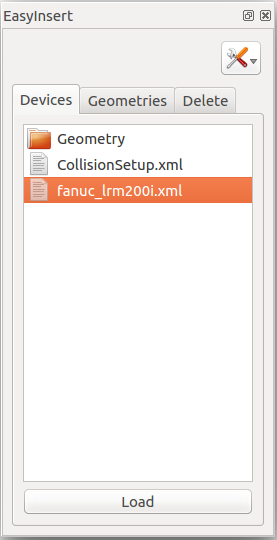
\includegraphics[width=.95\linewidth]{Figures/EasyInsertDevice.png}
  				\caption{Devices}
 				\label{fig:EasyInsertDevice}
        \end{subfigure}%
        \begin{subfigure}[b]{0.32\textwidth}
                \centering
                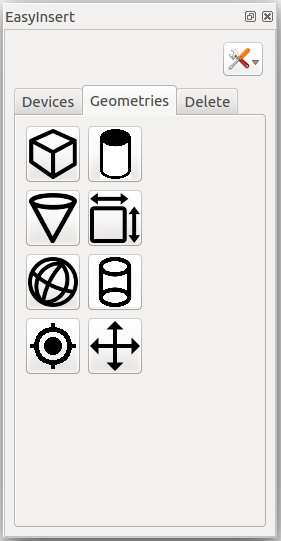
\includegraphics[width=.95\linewidth]{Figures/EasyInsertGeo.png}
  				\caption{Geometries}
  				\label{fig:EasyInsertGeo}
        \end{subfigure}%
        \begin{subfigure}[b]{0.32\textwidth}
                \centering
                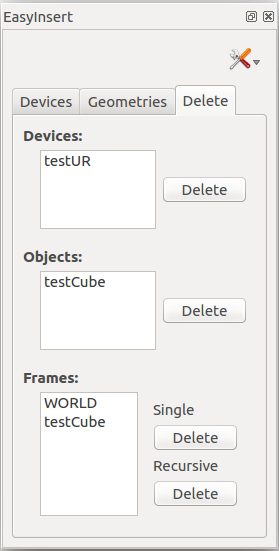
\includegraphics[width=.95\linewidth]{Figures/EasyInsertDelete.png}
  				\caption{Delete}
  				\label{fig:EasyInsertDelete}
        \end{subfigure}%
        \caption{The three tabs a user can interact with in the plugin. In Devices it is possible to select and load a device. In Geometries the user can click an icon (representing a geometry) which then prompts a dialog window with options regarding the insertion of said geometry. In Delete a user can select either a Device, Object or Frame to delete it.}\label{fig:EasyInsertTabs}
\end{figure}

It should be noted, that the first time EasyInsert is loaded and opened, the list shows the root content of the operating system. Thus the user need to change the path of the list shown in the Device tab to a path containing any desired devices. In the right top corner of the plugin is a settings button(a orange wrench and screwdriver), clicking this button and choosing Libraries will prompt the user with dialog window on Figure~\ref{fig:settingsDialog}. The user can here see what path is used and change it with the [...] button. The [...] button shows a new dialog window where the user can navigate his OS and specify the path that should be shown in the device tab.

\begin{figure}[h] % 3 figures of dialog windows
     \centering
     \begin{subfigure}[b]{0.45\textwidth}
	  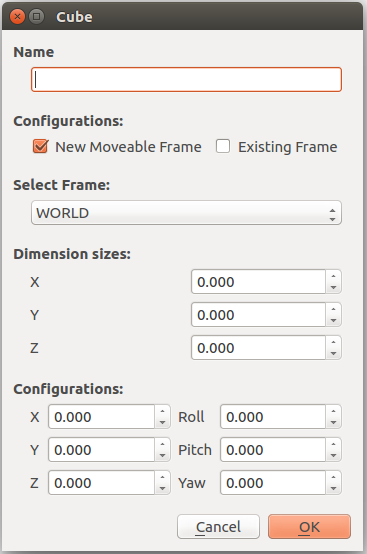
\includegraphics[scale=0.7]{Figures/EasyInsertCubeDialog.png}
       \caption{Cube insertion dialog window}\label{fig:cubeDialog}
     \end{subfigure}
     \hfill
     \begin{minipage}[b]{0.45\textwidth}
       \begin{subfigure}[b]{\linewidth}
	    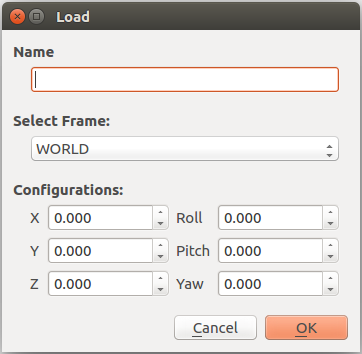
\includegraphics[scale=0.7]{Figures/EasyInsertLoadDialog.png}
         \caption{Device insertion dialog window}\label{fig:loadDialog}
       \end{subfigure}\\[\baselineskip]
       \begin{subfigure}[b]{\linewidth}
	    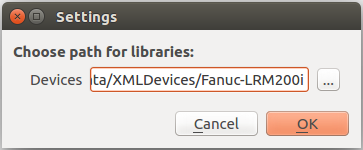
\includegraphics[scale=0.7]{Figures/settingsDialogWindow.png}
         \caption{Settings of device path dialog window}\label{fig:settingsDialog}
       \end{subfigure}
     \end{minipage}
     \caption{Three, out of many, dialog windows the user can experience and interact with when using EasyInsert.}\label{fig:EasyInsertDialogs}
\end{figure}

The Geometries tab shows a grid of icons, see figure~\ref{fig:EasyInsertGeo}. These icons represent either geometric primitives or frames that can be inserted into the WorkCell. Currently there are the following objects in the geometric tab, from top row to bottom:
\begin{enumerate*}[font={\color{red!50!black}\bfseries}]
\item Cube.
\item Cylinder.
\item Cone.
\item Plane.
\item Sphere.
\item Tube.
\item Fixed frame.
\item Movable frame.
\end{enumerate*}
These icons are all buttons the user can click, and after a click has occurred a dialog window appears with options regarding the insertion of said geometry. When the user hovers over a button, a small box identifying the icon appears, telling the user what sort of object it is. Figure~\ref{fig:cubeDialog} is the dialog window prompted when clicking the cube icon, and as seen, the user can specify a name for the geometry, select a reference frame and set the displacement and rotation configurations, just like when inserting a device. Though for a geometric primitive, like the cube, the user can also specify the dimensions of the geometric figure. The user can also specify whether the primitive should create a movable frame to associate the object with, or if the user want to use an existing frame.


\subsection{Dialog Windows}
The dialog window is the main communication with the user in this plugin. Dialog windows are top-level windows, and they provide the user with either information, or they allow the users to select options to perform a command or task. This section will show how dialog windows has been handled in the plugin.\\

The dialogs of EasyInsert has been implemented in it's own class dialog.hpp, i.e. a subclass of QDialog, see figure~\ref{fig:subClassQWidget} for an example of a Qt subclass. This was done to keep it independent and self-contained from the rest of the plug-in. The constructor for the dialog class is very simple, see figure~\ref{fig:dialogConstructor}. A constructor with no WorkCell parameter is also available and passing a parent is optional, though a name must always be given to the constructor. 

\begin{figure}[h] % Code of dialog constructor
\centering
\lstset{language=C++} 
\begin{lstlisting}[frame=single]  
dialog::dialog(rw::models::WorkCell::Ptr wc, QString dialog, QWidget *parent)
    : QDialog(parent)
{
    _workCell = wc;
    mainLayout = new QVBoxLayout();
    setWindowTitle(dialog);
}			 
\end{lstlisting}
\caption{The dialog class constructor. A WorkCell pointer to a RW instance is passed along as a parameter. The QString parameter is the name of the dialog box and the QWidget is a pointer to the parent widget }
\label{fig:dialogConstructor} 	
\end{figure}

The dialog class is fairly simple to use and extend. A dialog is made of blocks in a vertical layout of QWidget's, i.e. a dialog instance is a composite widget containing composite widgets. Figure~\ref{fig:dialogWindowExample} shows a dialog window with four blocks initialised.

\begin{figure}[h]
	\centering
	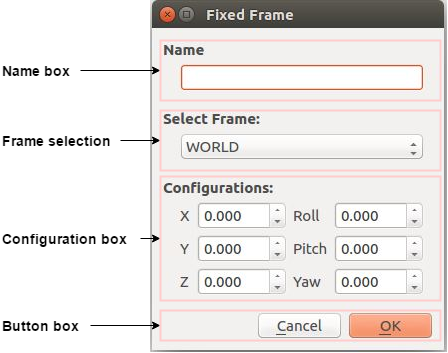
\includegraphics[scale=0.55]{Figures/dialogclassblocks.png}
	\caption{This figure shows a dialog window of adding a fixed frame to a WorkCell containing various widgets relevant to the action. }
	\label{fig:dialogWindowExample}
\end{figure}

All the blocks used to create all the dialog windows in the plug-in are shown in figure~\ref{fig:dialogBlocks}. These blocks are just member functions of the dialog class which returns a composite widget. So to create a dialog window as shown on figure~\ref{fig:dialogWindowExample}, a dialog instance should be constructed (in this case with a WorkCell pointer) and then simply adding the blocks to the dialog with the utility member function addToDialog(). See figure~\ref{fig:dialogWindowCode} which shows a code example on how to use the dialog class to construct the dialog window as shown on figure~\ref{fig:dialogWindowExample}. Since the dialog class is a subclass of QDialog, the position of the dialog window (opposed to a normal QDialog object) is always centred to the main application (RWS), even though a parent is passed as a parameter.

\begin{figure}[h] % code of adding stuff to a dialog
\centering
\lstset{language=C++} 
\begin{lstlisting}[frame=single]  
QString st = "Fixed Frame"; //Name of the dialog window
rw::models::WorkCell::Ptr wc = getRobWorkStudio()->getWorkCell(); //WorkCell
dialog* geoDialog = new dialog(wc,st,this); //Create the dialog window
geoDialog->addToDialog(geoDialog->createNameBox()); //Adding something
geoDialog->addToDialog(geoDialog->createFrameSelection());
geoDialog->addToDialog(geoDialog->createConfigurationBox());
geoDialog->addToDialog(geoDialog->createButtonBox());	
geoDialog->exec(); //execute/open dialog window	 
\end{lstlisting}
\caption{A sample code to illustrate how to construct the dialog window from figure~\ref{fig:dialogWindowExample}.}
\label{fig:dialogWindowCode} 	
\end{figure}

exec(), seen on figure~\ref{fig:dialogWindowCode} line 8, is an inherited public slot that executes/shows the dialog window. The dialog shown is in modal mode, meaning the window denies all user actions on any other widgets in the application. The function returns a DialogCode containing the information about whether the dialog window was accepted or rejected. The accepted or rejected information is determined by the user input to the createButtonBox() function block, since the OK button emits a accepted() signal to the accept() slot of the dialog object when pressed. Likewise the Cancel emits a rejected() signal to the reject() slot of the dialog object, though a rejected() signal is also emitted when the user presses ESC on the keyboard or the x(close) button of the dialog window. 

So when a dialog window has been created and used by a user, then some functionality should be executed based on the inputs given to the dialog. That means when the function exec() returns, we need to know whether the user accepted or rejected the dialog window (pressed OK or Cancel). This is done with the inherited public function result(). The function result() returns QDialog::Accepted when the dialog was accepted and QDialog::Rejected when it was rejected (QDialog::Accepted and QDialog::Rejected are both just normal enumerators, i.e. 1 and 0). 

\begin{figure}[h] % code of what to do after exec
\centering
\lstset{language=C++} 
\begin{lstlisting}[frame=single]  
geoDialog->exec();
if(geoDialog->result() == QDialog::Accepted) //Check the result
{
	std::string name = geoDialog->getNameBox(); //Get the name input
	std::string frame = geoDialog->getFrameSelection(); //Get frame selc
											 
		/*	Do something with the information    */ 
		
}
delete geoDialog; //Delete the dialog object when done using it
\end{lstlisting}
\caption{A sample code illustrating what to do after the exec()function returns.}
\label{fig:dialogAcceptedRejectedCode} 	
\end{figure}

As seen on figure~\ref{fig:dialogAcceptedRejectedCode}, after the exec() function returns, we simply check whether the result was QDialog::Accepted or not. If the result is accepted, then something should be done with the inputs given to the dialog window. We access these input via self explanatory public get-functions, e.g. the NameBox contains the name input (as seen on figure~\ref{fig:dialogAcceptedRejectedCode} line 4). After we have collected all the information we wanted out of the dialog window, then we can proceed to do something with the information, like e.g. the insertion of a frame. When we are done with the dialog window it should be deleted, because the dialog object is still alive until the parent is dead (in this case the plugin). If we do not delete the dialog object the dialog objects, created in the lifetime of the plugin, will just waste space in memory. 

It would take some time to inspect all of the function blocks on figure~\ref{fig:dialogBlocks}. Therefore only one function block, namely createNameBox() figure~\ref{fig:dialogCreateNameBoxCode} will be inspected. All the function blocks has a similar structure except from createLibSettingsBox(), which functionality will be discussed SOMEWHERE I DNO YET.

\begin{figure}[h] % code example of createNameBox
\centering
\lstset{language=C++} 
\begin{lstlisting}[frame=single]  
QWidget* dialog::createNameBox() {
    QGroupBox* nameBox = new QGroupBox(tr("Name")); //The nameBox widget
    QHBoxLayout *layout = new QHBoxLayout; //layout for the nameBox
    nameLine = new QLineEdit(); //The line edit the user can type the name
    layout->addWidget(nameLine); //Add the line edit to the layout
    nameBox->setLayout(layout); //Set the layout to the namebox
    return nameBox; //Return the nameBox
}
\end{lstlisting}
\caption{This figure shows the pulic function createNameBox() from the dialog class. The function is used to add a name line edit to dialog windows.}
\label{fig:dialogCreateNameBoxCode} 	
\end{figure}

The general procedure in the function blocks, as seen on figure~\ref{fig:dialogCreateNameBoxCode}, is to first create the composite widget. This widget, in the case of createNameBox, is a QGroupBox widget. QGroupBox is a widget that is mainly used as a composite widget. The QGroupBox provides a box to group widgets in, a frame if wanted and a title. As seen on figure~\ref{fig:dialogCreateNameBoxCode} line 2, the title is set upon construction with the string "Name". The tr() function is for translation purposes \cite{QtDocumentationTr}.
After the composite widget has been created, the layout for the parent widget has to be chosen and the child widget(s), in this case a QLineEdit(), has to be created. QLineEdit() is a simple line where text can be typed and edited in. When all the child widgets has been created, they need to be added to the layout of the parent. Lastly the layout is set to the parent and the parent is then returned. It should be noted that when the QLineEdit() was created, figure~\ref{fig:dialogCreateNameBoxCode} line 4, no parent was defined, i.e. it is actually not a child widget but a top-level widget. This is fine though, because when a top-level widget is added to a layout of another widget, that widget automatically takes responsibility as a parent and the top-level widget is now a child of that widget.

\begin{figure}[h] % table of function blocks
\centering
\begin{center}
  \begin{tabular}{ | l | p{7cm} |}
    \hline
    \textbf{Function blocks} 	   &   \textbf{Description}  \\ \hline
    createButtonBox()			   &   The Cancel and OK buttons. This block is used in all the dialog windows.   		\\ \hline
    createNameBox() 			   &   A line edit to specify a name.   		\\ \hline
    createCheckFramesBox()		   &   Two exclusive check boxes, i.e. only one of the boxes can be checked at a time.		\\ \hline
    createConfigurationBox() 	   &   The different configurations available to adjust regarding displacement and rotation of the inserted element. 		\\ \hline
	createConfigurationBoxCube()   &   A cube specific configuration option, i.e. the dimensions of the cube.  	\\ \hline	    
	createConfigurationBoxSphere() &   A sphere specific configuration option, i.e. the dimensions of the sphere. 	\\ \hline	
	createConfigurationBoxCone()   &   A cone specific configuration option, i.e. the dimensions of the cone.  	\\ \hline	
    createConfigurationBoxTube()   &   A tube specific configuration option, i.e. the dimensions of the tube.  	\\ \hline	
	createLibSettingsBox()		   &   This block is used to edit the settings of the device library.    	\\ \hline	 
	createFrameSelection()		   &   A way to select a parent frame for the inserted element. Default is the WORLD frame.		\\
    \hline
  \end{tabular}
\end{center}
\caption{This table summarizes all the different dialog function blocks used to construct the dialog windows in the plug-in.}
\label{fig:dialogBlocks} 
\end{figure}


Something about what could be worked on in regard to this class. Like constructors for a generic dialog window, mainlayout in a grid instead and extended adddialog functionality.
Is this something that should be in this chapter?






